\documentclass{article}

\usepackage{lipsum}
\usepackage{graphicx}
\usepackage{float}
\usepackage{pgfplots}
\usetikzlibrary{arrows}
\usepackage{caption}
\usepackage{tikz}
\usepackage{capt-of}
%Lay-out options
\usepackage{fancyhdr}
\pagestyle{fancy}
\fancyhead{}
\fancyfoot{}
\fancyfoot[R]{ Page : \thepage\ }
\renewcommand{\headrulewidth}{0pt}






\begin{document}
% Title page
\begin{titlepage}
    \begin{center}
   
    \huge{\bfseries Numerical Simulation Assignment 2}
    \line(1,0){300}\\
    [1.5cm]
    \textsc{\Large Economics of Risk and Time in Latex}\\
    [12cm]
    \end{center}
    \begin{flushright}
    \textsc{\large by: N.A. Goedhart \\
    ANR: 405071 \\
    March 15, 2016 \\}
    \end{flushright}
\end{titlepage}
\pagenumbering{roman}
%\section*{Summary}
%\addcontentsline{toc}{section}{\numberline{}Summary}
%\cleardoublepage
%\section*{met dank aan}
%\addcontentsline{toc}{section}{\numberline{}Aknowledgements}
%\cleardoublepage
%Inhoudsopgave
\tableofcontents
\thispagestyle{empty}
\cleardoublepage

%list of figures
\setcounter{page}{1}
\listoffigures
\addcontentsline{toc}{section}{\numberline{}List of Figures}
\cleardoublepage





%Introductie
\newpage
\pagenumbering{arabic}
\setcounter{page}{1}

\section{Introduction}\label{sec:intro}
In this document I present two exercises that were in assignment 2 from Seminar Economics of Risk and Time (2016). This assignment was originally made by: me, Edgar Brouwer, Jonathan Koets, Jules Perry and Arjan Spaans. This assignment has not yet been graded or corrected. By this no rights can be derived from this document.
%Inhoud
\newpage
\section{Exercises}
\subsection{Exercise 1}
Consider an urn with 9 balls: 3 balls are red and the remaining 6 balls are either all green or all yellow. Thus, the urn contains 3 red and 6 greens balls, or 3 red and 6 yellow balls. One ball will be drawn at random from the urn. Consider the prospects A = (R: �100; Y: �0; G: �0), B = (R: �0; Y: �100; G: �0), C = (R: �100; Y: �0; G: �100), and D = (R: �0; Y: �100; G: �100), where R, Y, and G denote the event that a red, yellow, and green ball will be drawn from the urn.
\subsubsection{Exercise 1.a.}
a) It has been found that most people prefer prospect A to B, while they simultaneously prefer prospect D to prospect C. Show that this choice pattern violates Subjective Expected Utility.\\
[0.5cm]

SEU(L) = $\displaystyle \sum_{i}{B(Ei)}{u}{Xi}$\\

\ SEU(A) = $\displaystyle\frac{3}{9}\times0+\frac{1}{2}\times\frac{6}{9}\times0+\frac{1}{2}\times\frac{6}{9}\times0=33\frac{1}{3}$\\

\ SEU(B) = $\displaystyle\frac{3}{9}\times0+\frac{1}{2}\times\frac{6}{9}\times100+\frac{1}{2}\times\frac{6}{9}\times0=33\frac{1}{3}$\\

\ SEU(C) = $\displaystyle\frac{3}{9}\times100+\frac{1}{2}\times\frac{6}{9}\times0+\frac{1}{2}\times\frac{6}{9}\times100=66\frac{2}{3}$\\

\ SEU(D) = $\displaystyle\frac{3}{9}\times0+\frac{1}{2}\times\frac{6}{9}\times100+\frac{1}{2}\times\frac{6}{9}\times100=66\frac{2}{3}$\\

Since SEU(A)=SEU(B) and SEU(C)=SEU(D) people should be indifferent between choosing prospect A and B and between choosing prospect C and D.

\subsubsection{Exercise 1.b.}
b) Show that the $\alpha$-MEU model can accommodate the majority choice.\\
[0.5cm]
\ $\alpha$-MEU( f )=$\alpha$minp$\epsilon$C(Ep[u( f )]) + (1-$\alpha$)maxp$\epsilon$C(Ep[u( f )])\\
$\alpha$= 0.8\\
[0.5cm]
\ $\alpha$-MEU(A) = $\frac{1}{3}\times100 = 33\frac{1}{3}$\\
[0.125cm]
\ $\alpha$-MEU(B) = $\frac{4}{5}\times(0\times100)+(1-\frac{4}{5})\times(\frac{2}{3}\times100) = 13\frac{1}{3}$\\
[0.125cm]
\ $\alpha$-MEU(C) = $\frac{4}{5}\times(\frac{1}{3}\times100)+(1-\frac{4}{5})\times(1\times100) = 13\frac{1}{3}$\\
[0.125cm]
\ $\alpha$-MEU(D) = $\frac{2}{3}\times100 = 66\frac{2}{3}$\\
\cleardoublepage
Since $\alpha$-MEU(A) $>$ $\alpha$-MEU(B) and $\alpha$-MEU(D) $> \alpha$-MEU(C) the $\alpha$-MEU model can accommodate the majority choice.\\
\subsubsection{Exercise 1.c.}
c) Show that the Recursive Expected Utility model can accommodate the majority choice.\\
\ REU( f ) = E$\mu$[$\phi$(Ep$\epsilon$C[u( f )])]\\
[0.25cm]
$\phi = x^{0.5}$\\

\ REU(A) = $\displaystyle(\frac{1}{3}\times100)^{\frac{1}{2}}=5.77\\$

\ REU(B) = $\displaystyle\frac{1}{2}\times(\frac{2}{3}\times100+\frac{1}{3}\times0)^{\frac{1}{2}} + \frac{1}{2}\times(0\times100+\frac{2}{3}\times0+\frac{1}{3}\times0)^{\frac{1}{2}} =4.08\\$

\ REU(C) = $\displaystyle\frac{1}{2}\times(\frac{1}{3}\times100+\frac{2}{3}\times100)^{\frac{1}{2}} + \frac{1}{2}\times(\frac{1}{3}\times100+\frac{2}{3}\times0)^{\frac{1}{2}} =7.88\\$

\ REU(D) = $\displaystyle\frac{1}{2}\times(\frac{2}{3}\times100)^{\frac{1}{2}} + \frac{1}{2}\times(\frac{2}{3}\times100)^{\frac{1}{2}} =8.16\\$

Since $REU(A)>REU(B) and REU(D)>REU(C)$ recursive expected utility can accommodate the majority choice.\\
\cleardoublepage
\subsection{Exercise 2}
When choosing between uncertain alternatives, Mary maximizes cumulative prospect theory with a weighting (source) function for a ball drawn from an urn with a known composition of balls (K) equal to the weighting function for the performance of the Dow Jones index, both given by: $wK(p)=wDOW(p)=p^2$. The weighting function for balls drawn from an urn with an unknown composition of colored balls (U), as well as the weighting function for the performance of the AEX index are given by $wU(p)=wAEX(p)=\frac{p^{0.5}}{((p^{0.5}+(1-p)^{0.5})^2)}$. Mary's utility function is $u(x)=x^{0.88}$.\\
\subsubsection{Exercise 2.a.}
a)Show that Mary can be ambiguity seeking for unlikely events and ambiguity averse for events of moderate likelihood when comparing lotteries with prizes depending on balls drawn from either the risky or the unknown urn.\\

\begin{center}
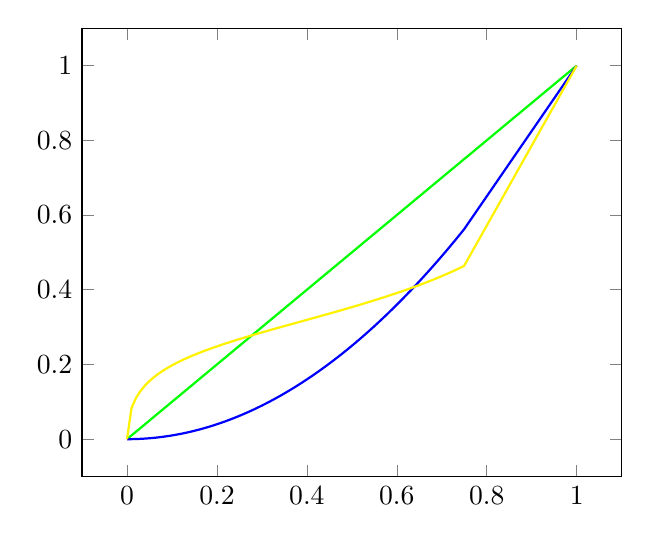
\begin{tikzpicture}
    \begin{axis}[samples at={0,0.01,...,0.75,1}]
       \addplot[green,thick]{(x)};
       \addplot[blue,thick]{(x)^(2)};
       \addplot[yellow,thick]{(x^0.5)/((x^0.5+(1-x)^0.5)^2)};
    \end{axis}
    \label{fig:Plotted weighting functions}
\end{tikzpicture}
\captionof{figure}{Graph of weighting functions}


Figure \ref{fig:Plotted weighting functions} Comparison of weighting functions
\end{center}
The above graph shows the statements made in the question. If we look at probabilities close to zero (say $<0.3$) Mary prefers to bet on the unknown urn compared to the risky urn since she over-weights the small probabilities since they are above the $45^0$ line (especially for probabilities that are close to zero). When the probabilities are moderate to high Mary prefers to bet on the risky urn however for both the unknown urn as for the risky urn she under-weights the probabilities since they are below the $45^0$ line.\\
\subsubsection{Exercise 2.b.}
b) Show that Mary can exhibit the home bias, assuming that she beliefs that the Dow Jones index and the AEX index will go up (and down) with probability 0.5.\\
In this case Mary gains \$100 dollar if the AEX or the Dow Jones will go up:\\ 

\ $wK(0.5)=0.25; wU(0.5)=0.3535$

\ $wK(0.5)\times100=25; wU(0.5)\times100=35.35$

\ $u(25)=16.99; u(35.35)=23.05$

From this it shows that although the probability for both stock exchanges to go up is equal, Mary is more willing to invest in the AEX index. If Mary is Dutch, this is a case of the Home Bias.\\








\end{document}

